\documentclass{standalone}

\usepackage[euler-digits]{eulervm}

\usepackage{tikz}
\tikzset{every node/.style={draw=none,minimum size=2mm,inner sep=0pt}}

\begin{document}
    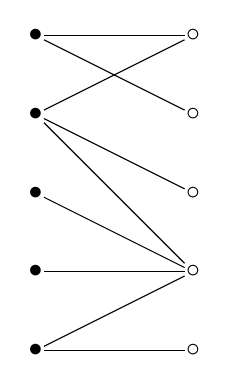
\begin{tikzpicture}[scale=1]
      \node (1) at (-1,4) {$\bullet$};
      \node (2) at (-1,3) {$\bullet$};
      \node (3) at (-1,2) {$\bullet$};
      \node (4) at (-1,1) {$\bullet$};
      \node (5) at (-1,0) {$\bullet$};
      \node (v) at (1,4) {$\circ$};
      \node (w) at (1,3) {$\circ$};
      \node (x) at (1,2) {$\circ$};
      \node (y) at (1,1) {$\circ$};
      \node (z) at (1,0) {$\circ$};

\foreach \a/\b in {1/v,1/w,2/v,2/x,2/y,3/y,4/y,5/y,5/z}
  \draw (\a) -- (\b);
    \end{tikzpicture}
\end{document}
